\documentclass[12pt,a4paper,fleqn]{article}
\title{Progress Report}
\author{Syed Ahmad Raza\\
        D10503816}
\date{2018.12.05}
\usepackage{mathtools}          % for math
\usepackage{graphicx}           % for graphics
\usepackage{booktabs}           % for professional tables
\usepackage{float}              % force a figure placement with [H] command
\usepackage{newtxtext}          % better text font
\usepackage{newtxmath}          % better math font
\usepackage{nicefrac}           % use nicer smaller fractions
\graphicspath{{../figures/}}    % only works when -shell-escape is used with pdflatex
%\usepackage{enumitem}           % control layout of itemize and enumerate
%\usepackage{layouts}            % find \printinunitsof{in}\prntlen{\textwidth}
%\usepackage{xcolor}             % for using colors in document

\begin{document}
\maketitle
%\tableofcontents
%\pagebreak

\section{Implementation of direct-forcing immersed boundary method (DFIB) in C++ using finite volume method with subgrid method}

The three-dimensional solver for Navier-Stokes equations has been modified to implement direct-forcing immersed boundary method. A test case was run for a small cubic cavity with a sphere in the middle. The diameter of the sphere is half the length of the sphere. The size of the computational grid for this test case is \(20 \times 20 \times 20\) with a subgrid of \(10 \times 10 \times 10\) for the solid sphere. Another test case was run with a nonuniform grid of \(16 \times 16 \times 16\) and a subgrid of \(20 \times 20 \times 20\).

\subsection{Results}

\begin{figure}[H]
    \centering
    \includegraphics[width=\linewidth]{virtualForceVectors.png}
    \caption{Virtual force vectors, \(\eta \boldsymbol{f}\), plotted on the surface of the sphere in a cubic cavity with \(20 \times 20 \times 20\) grid.}
\end{figure}

\begin{figure}[H]
    \centering
    \includegraphics[width=\linewidth]{velocityVectors.png}
    \caption{Velocity vectors plotted around the sphere in a cubic cavity with a \(20 \times 20 \times 20\) grid.}
\end{figure}

\begin{figure}[H]
    \centering
    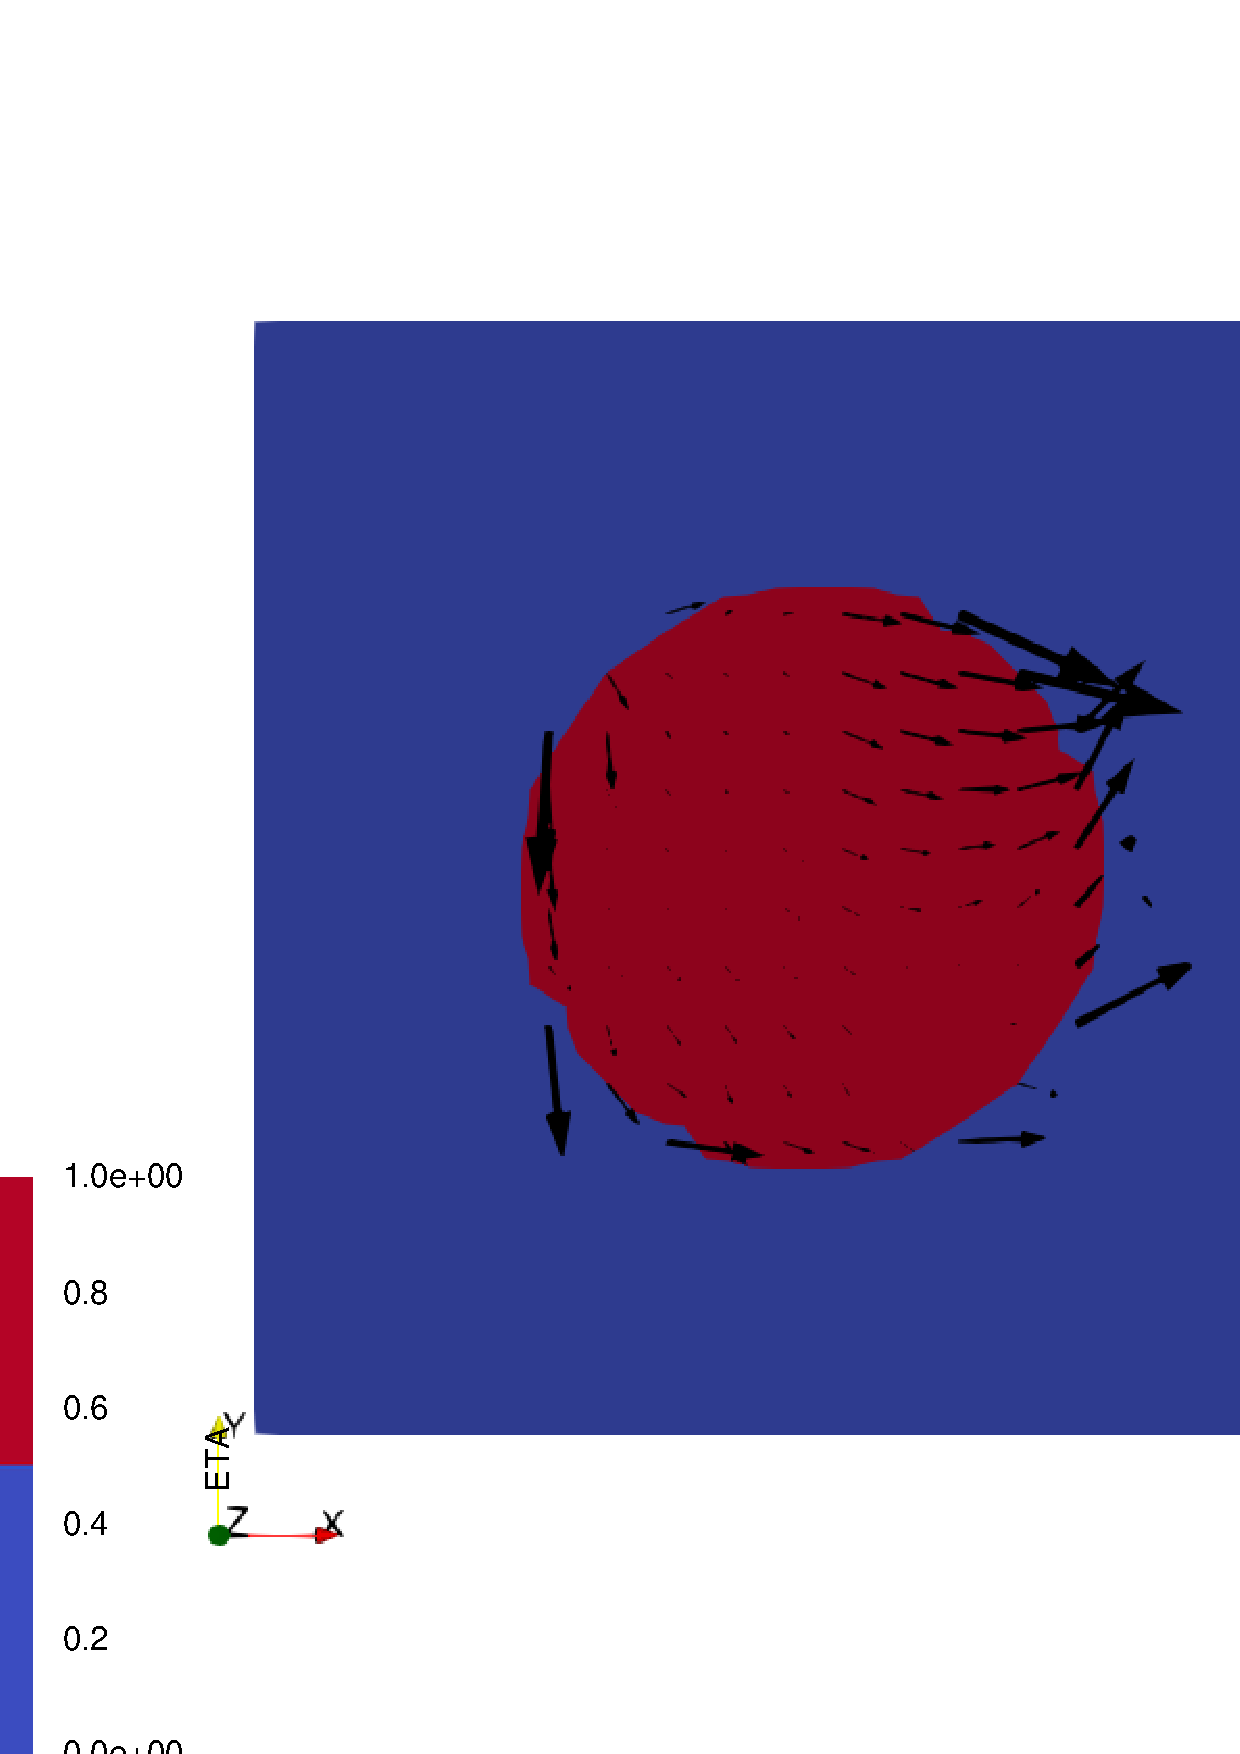
\includegraphics[width=\linewidth]{planarVirtualForceVectors.png}
    \caption{Virtual force vectors, \(\eta \boldsymbol{f}\), plotted on the \(xy\)-plane at the center of the cubic cavity with a \(20 \times 20 \times 20\) grid.}
\end{figure}

\begin{figure}[H]
    \centering
    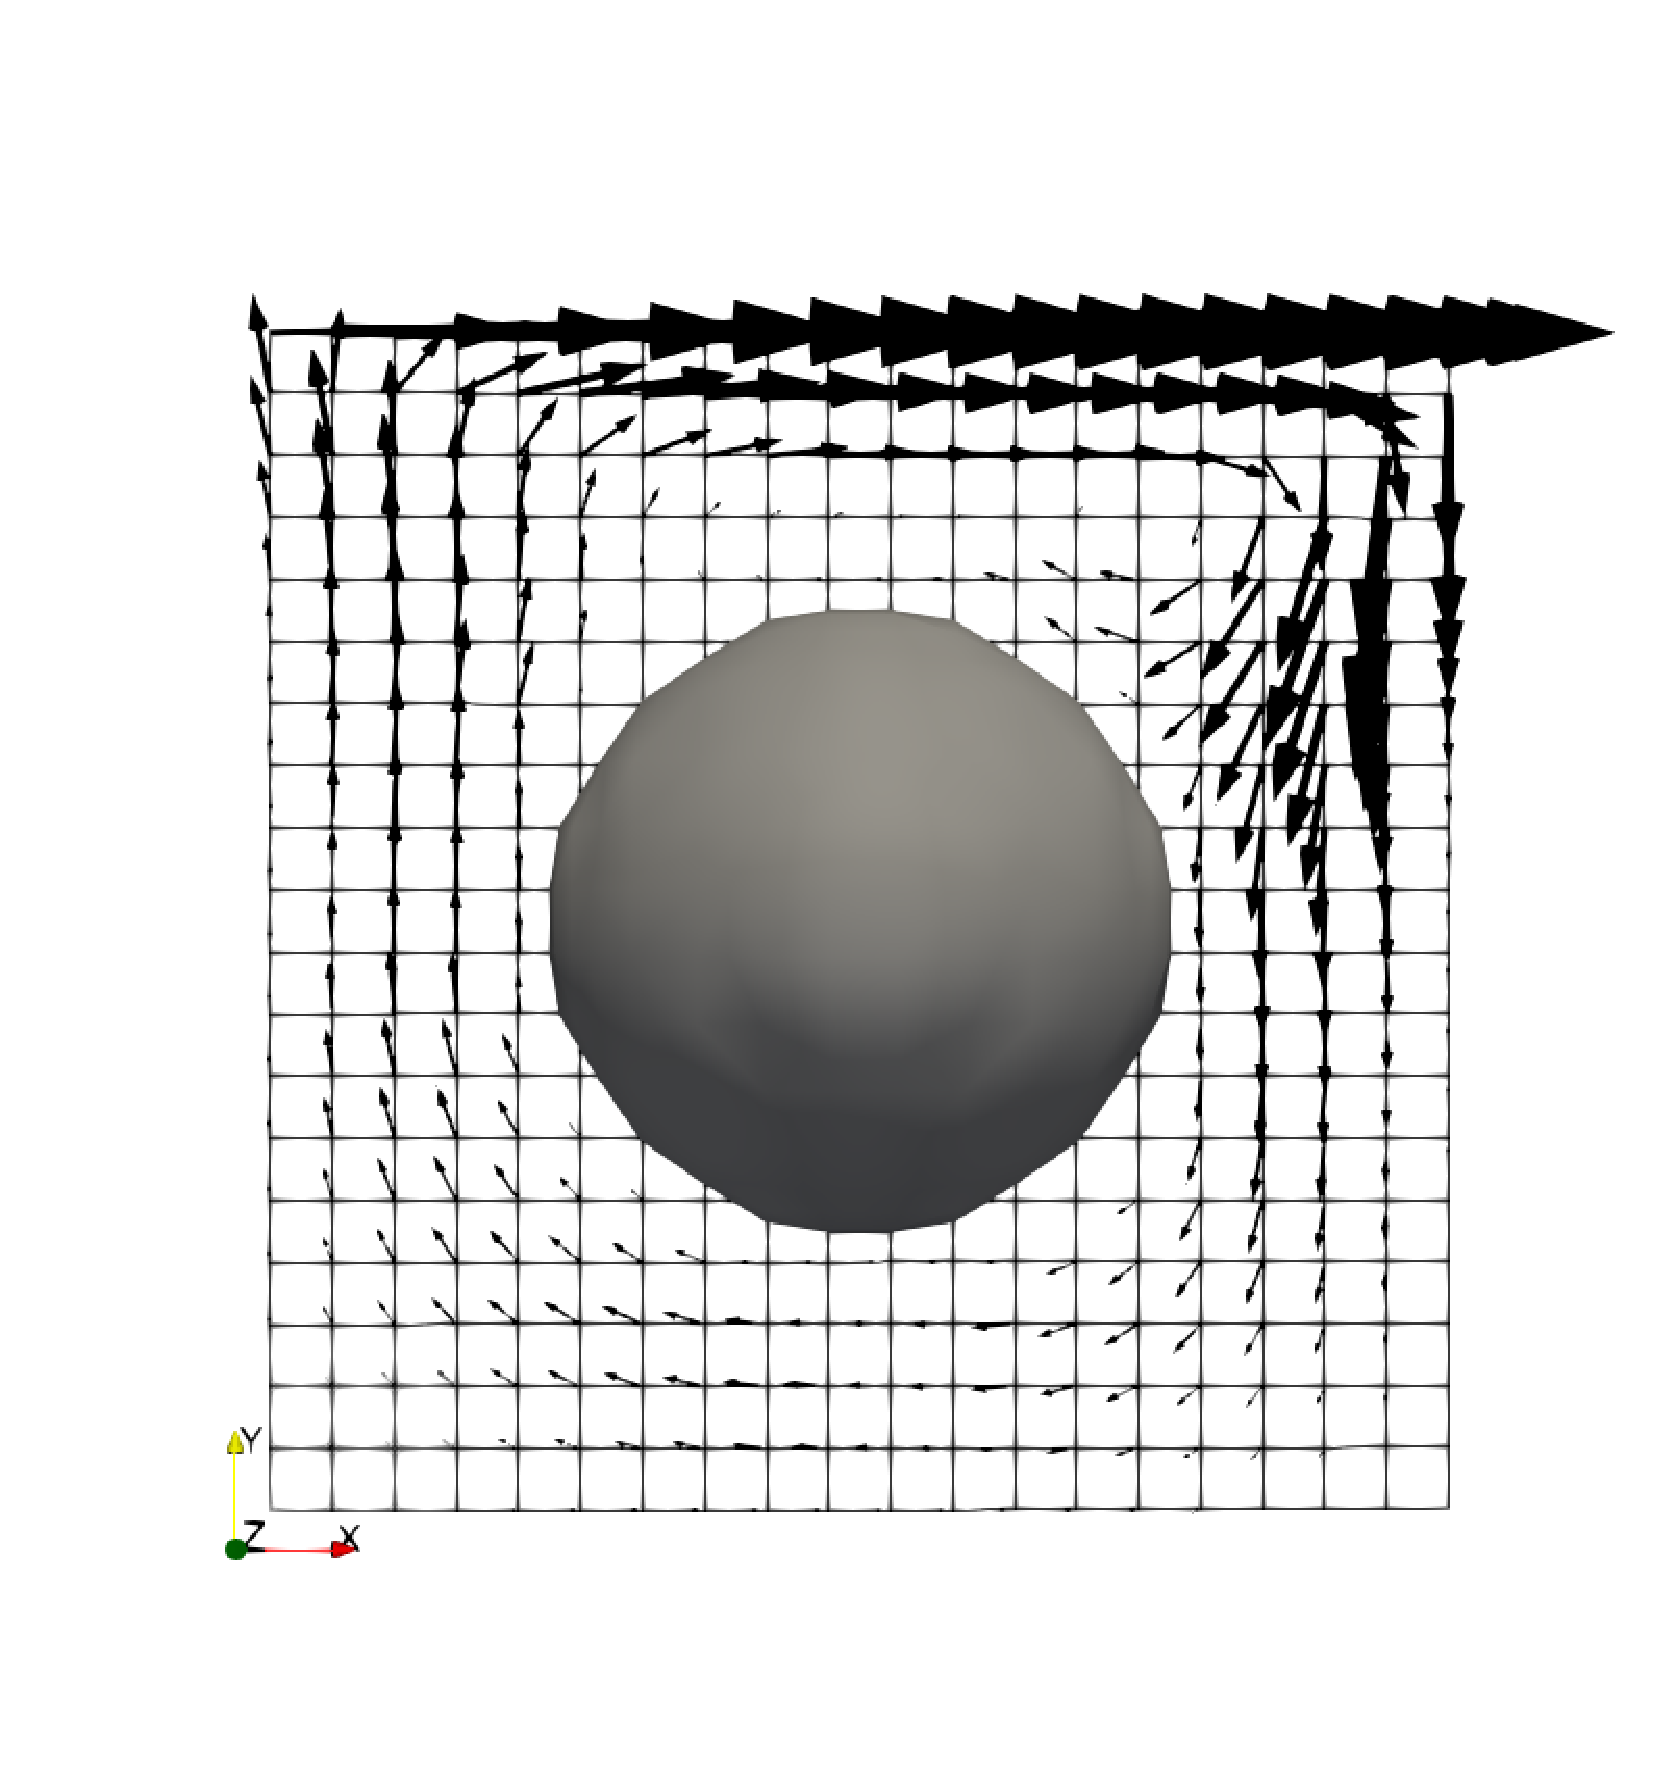
\includegraphics[width=\linewidth]{planarVelVectors.eps}
    \caption{Velocity vectors plotted on the \(xy\)-plane at the center of the cubic cavity with a \(20 \times 20 \times 20\) grid.}
\end{figure}

\begin{figure}[H]
    \centering
    \includegraphics[width=\linewidth]{sphereContour_nonuniformGrid.png}
    \caption{Velocity vectors plotted on the \(xy\)-plane at the center of the cubic cavity with a \(16 \times 16 \times 16\) grid.}
\end{figure}

\subsection{Future work}
\begin{itemize}
    \item Implement model equations for vortex-induced vibration.
\end{itemize}

\newpage
% References
%\bibliographystyle{unsrt}
%\bibliography{BIB_WENO-1997-Shu_Book-Advanced_Numerical_Approximation.bib}

\end{document}
